\chapter{Approach}
\label{methodology}

% \begin{itemize}
%     \item Explain the data collection step, and how the comments were collected and aligned using BinSwarm. 
%     \item Explain the deduplication methods used and why duplicates in this task are fine, but why we choose to report the deduplicated results anyway.
%     \item Explain the experimental setup for the standard model, how we pre-processed the data, fed it into the model and the evaluation 
%     \item Explain the experimental setup for the pre-training, the translation, DOBF and span detection, how and why the pre-training steps were done, and how they were evaluated
% \end{itemize}
% \newpage
The proposed solution starts with a data collection step, where we collect open-source projects. These open-source projects are then compiled and decompiled. The decompiled functions are aligned with the documentation extracted from the source code. This data is then processed to extract descriptive comments and split into multiple sets. Finally, we use this data to fine-tune and evaluate a pre-trained CodeT5 model. We also design a few intermediate-training objectives, which are applied to the model before fine-tuning to improve the model performance. 

% \todo[inline]{you can include a running example to walk the reader through your approach, it makes it much easier to understand the work}

\section{Data Collection}
We require a dataset of decompiled functions labelled with a description to create and assess our solution. This dataset should be relatively large to suit the "data-hungry" nature of our deep-learning models. Furthermore, the dataset needs to feature a diverse set of data representative of our solution's actual real-life use case. 
To create a large and diverse dataset to train and assess our solution we made use of BinSwarm~\cite{InlinedFunc}, an existing dataset of aligned decompiled and stripped decompiled functions. \footnote{BinSwarm; \url{https://hub.docker.com/r/binswarm/cbuilds}}

Buildswarm starts by collecting C-based projects from Github. The projects are filtered to only include projects that are: Actively being developed, using Travis CI and built for Ubuntu Linux. The projects are built using Docker. The resulting binaries are then copied and stripped, and both the stripped and unstripped binaries are decompiled using Ghidra. The functions are extracted from the stripped and unstripped decompiled code and aligned with the source code. 
We extract documentation from the original source code to add descriptive comments to this dataset. We depend on the documentation included in the source code by the original authors in the form of single and multiline comments. The decompiled functions are aligned with the comments in the source code by using srcML to extract any documentation located directly before a function signature and then finding the function signature and project name in the decompiled dataset.

A function's documentation often also contains other details besides the descriptive summary. We found that C projects do not follow a single documentation standard. For example, Javadoc for Java has a short one-line description or summary for each method at the beginning of the multiline comment block. In C, there is no singular documentation standard, so there might not be a single line summary, and we will need to locate it in the comment block automatically. 
Furthermore, we found that a large number of functions did not have any documentation associated with them at all. To deal with these issues, we did not include any functions that are missing documentation. We devised a few simple rules to extract the summary to find the single sentence description.

A high-level overview of this process can is found in figure \ref{fig:dataCollection}.

\begin{figure}[!h]
  \centering
  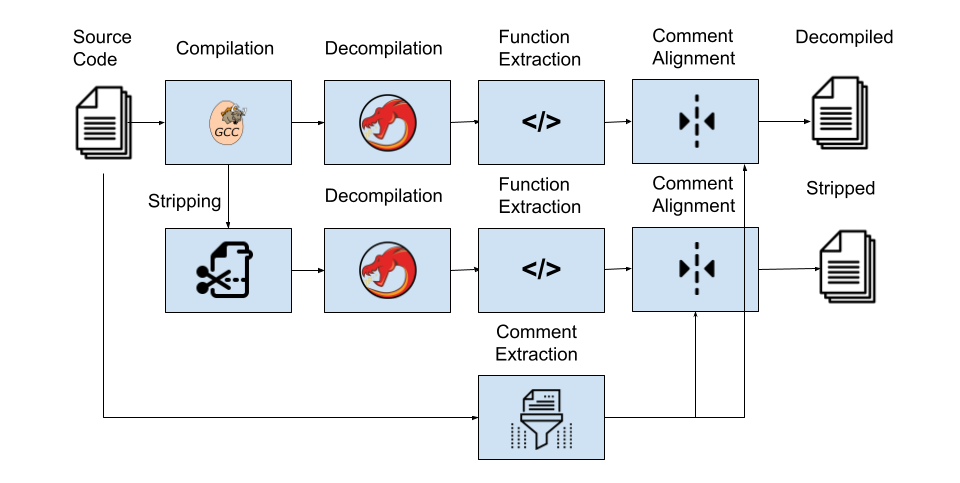
\includegraphics[width=\linewidth]{img/dataCollection.png}
  \caption{Data Collection}
  \label{fig:dataCollection}
\end{figure}

From the dataset of decompiled functions, another dataset is also created. We can emulate the process of stripping by removing all the identifiers from the decompiled code and replacing them with placeholders. For clarity, we call this demi-stripped data. Like the stripped dataset, the identifiers are all removed, but the decompiler still had access to the identifiers and could use the symbol table during decompilation. Most importantly, this demi-stripped dataset still has the same structure and control flow as the unstripped decompiled dataset.

\subsection{Dataset Split}
The dataset is split into a train, test and validation set. These sets constitute approximately, 80\%, 10\% and 10\% respectively\cite{recommend_summarization} of the complete dataset. To prevent leakage of vocabulary and code patterns between the sets, we sample the sets in a cross-project manner. This means that an entire project gets assigned to one of the sets, and functions from the same project cannot be assigned to different sets. The different sets should also have a similar distribution of optimisation level and average source-code length.

\subsection{Duplication}
Large corpora of code, like the corpus gathered by BinSwarm, tend to have a high degree of duplication~\cite{recommend_summarization}. As a result, snippets of code that are relatively unchanged appear in multiple parts of the corpus. This can be in the form of copied, generic or auto-generated functions. These functions will appear in multiple repositories and might be duplicated across the training and testing data.

Besides exact duplicates, near-duplicates can also occur. Near-duplicates are like exact duplicates, but they differ in a few minor aspects like additional code comments or different function names. While removing exact duplicates is relatively fast and straightforward, removing near-duplicates is much more challenging and computationally intensive~\cite{allamanis_adverse}. 

The issue with code duplication in classical code summarization is that the models and tools are supposed to be used to generate summaries for new and unseen code. The evaluation metrics should therefore measure the generalisation of the tool on new samples~\cite{allamanis_adverse}. Duplicates and near-duplicates are not defined as new samples. A user of such a tool could simply look these samples up. Furthermore, large, high-capacity models like CodeT5 with 220 million~\cite{CodeT5} or Codex with 12 billion~\cite{CodeX} trainable weights, have a large capacity to memorize duplicated code~\cite{allamanis_adverse}.
However, the use case outlined in this work is more akin to deobfuscation. As explained by~\citeauthor{allamanis_adverse}, deobfuscation could be a use case where duplicates are valid and part of the true distribution of the problem\cite{allamanis_adverse}. Unfortunately, compiled code contains a lot of duplicate code, and understanding this code is still difficult and essential for understanding the binary. We, therefore, focus on the model's performance on code with duplicates, but we also report the deduplicated results.

\section{Intermediate-Training}
The standard CodeT5 model was not pre-trained on any decompiled code. It might therefore be useful to apply additional training steps to 'teach' the model the embedding of decompiled and stripped decompiled code. Since we apply these training steps between the pre-training and fine-tuning of the model, we refer to this training strategy as intermediate-training.

To apply and assess other intermediate-training objectives, we train a CodeT5-base model on a predefined objective. Then after that intermediate-training step, we fine-tune the resulting model on our fine-tuning datasets. We essentially apply another training step to the already pre-trained base model. We can then measure the impact of the intermediate-training step on the model's performance after fine-tuning.

\begin{figure}[H]
  \centering
  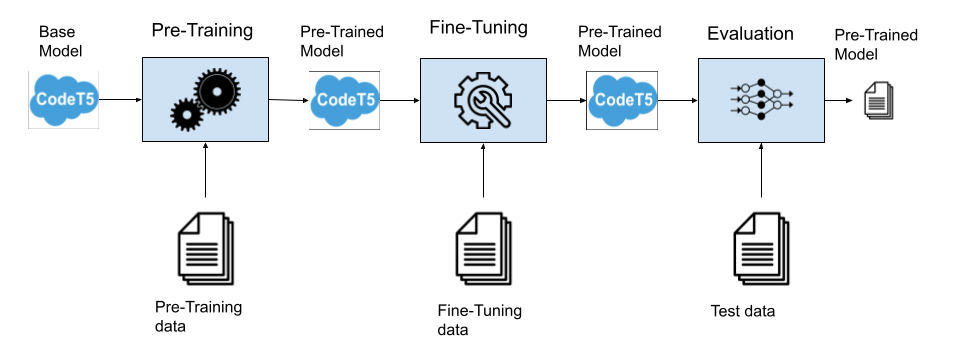
\includegraphics[width=\linewidth]{img/pre-training.png}
  \caption{Pre-Training}
  \label{fig:preTraining}
\end{figure}

We define several different pre-training objectives. Each of these objectives aims to teach the model the embedding of the identifiers, such that these identifiers can be inferred from the stripped code. For these objectives, we use the relatively large dataset of demi-stripped code. Some samples might be included in both the fine-tuning data and the intermediate-training data, but the model objective will differ. To prevent leakage, we remove the test set of the fine-tuning data from the intermediate-training data. 

\section{Fine-Tuning}
The concept of transfer learning, which is utilised in CodeT5, depends on the use of a fine-tuning step to train the pre-trained model on the downstream task. In this case, we make use of the CodeT5-base model, which was trained on mixed upstream tasks by the authors~\cite{CodeT5}.

We fine-tune a pre-trained CodeT5-base model on the constructed dataset. The model is trained on the summarization task as defined in the model. The model is trained on the train set, then evaluated after every epoch on the validation set and finally tested on the test set. During training, the performance of the model is measured using the BLEU-4 metric. BLEU-4 is reported to be unreliable when considering small changes in reported scores~\cite{CodeSumMetrics}. We further evaluate the performance using the EM (exact match), METEOR and ROUGE-L metrics.

